%!TEX root = ../thesis.tex
\subsection{User Evaluation}

To evaluate the usability and utility of DemoCut, we recruited 8 participants (4 males, ages 20-41) to create how-to video tutorials.
%Each participant video recorded himself or herself performing a task and edited the recording with DemoCut.
%md: removing this sentence because it's repetitive
We were especially interested in two questions: First, how much {\em effort} would participants have to invest to mark and edit their own tutorial videos with DemoCut? And second, what are the {\em qualities of the resulting videos} -- both in terms of strengths and shortcomings?
%We gathered
%, we invited participants to perform and film a physical demonstration of a common daily task in our lab setting. Users were asked to generate a video How-To tutorial using our system. We measured the performance of the system suggestions and how these meet participants' expectation.
%\subsection{Hypotheses}
%The goal of our user study was to understand if amateurs would be able to produce video tutorials that satisfied two hypotheses: 1) The final video output provided certain quality similar to current practices, and 2) The production required relatively short amount of time than editing from the raw footage.
% \pc{claim: from the user study, editing takes 1 hour to 1 day}.
%\bh{I'm downplaying the hypotheses since our n is relatively small and we'll probably rely more on qualitative data.}

\subsubsection{Task and Materials}
The participants were asked to create a tutorial for wrapping and decorating a present. We chose this task because it is relatively simple but still involves multiple distinct activities and steps that can be accomplished in 5-15 minutes. Possible steps include: measuring the gift size, cutting paper and ribbons, folding and wrapping, and decorating the present with ornaments.
%Multiple tutorial steps ensured that the tutorial would offer opportunities for several video editing decisions.
We offered the following supplies:
%, and the participants were free to use any of them.
\begin{itemize}
  \item \emph{Present}: a rectangular gift box of size $9 \times 2 \times 4.5$ inches.
  \item \emph{Tools}: scissors, utility knife, ruler, pencil, double-sided tape, transparent tape, and glue.
  \item \emph{Wrapping paper}: a variety of wrapping paper rolls including plain, patterned, and textured.
  \item \emph{Decorations}: ribbons (curling and fabric) in multiple colors, gift bows, stickers, and message cards.
\end{itemize}
To help them understand the context of the study, the participants were asked to watch three videos before visiting our lab. The videos were selected from the formative user study.

\begin{figure}[t]
  \centering
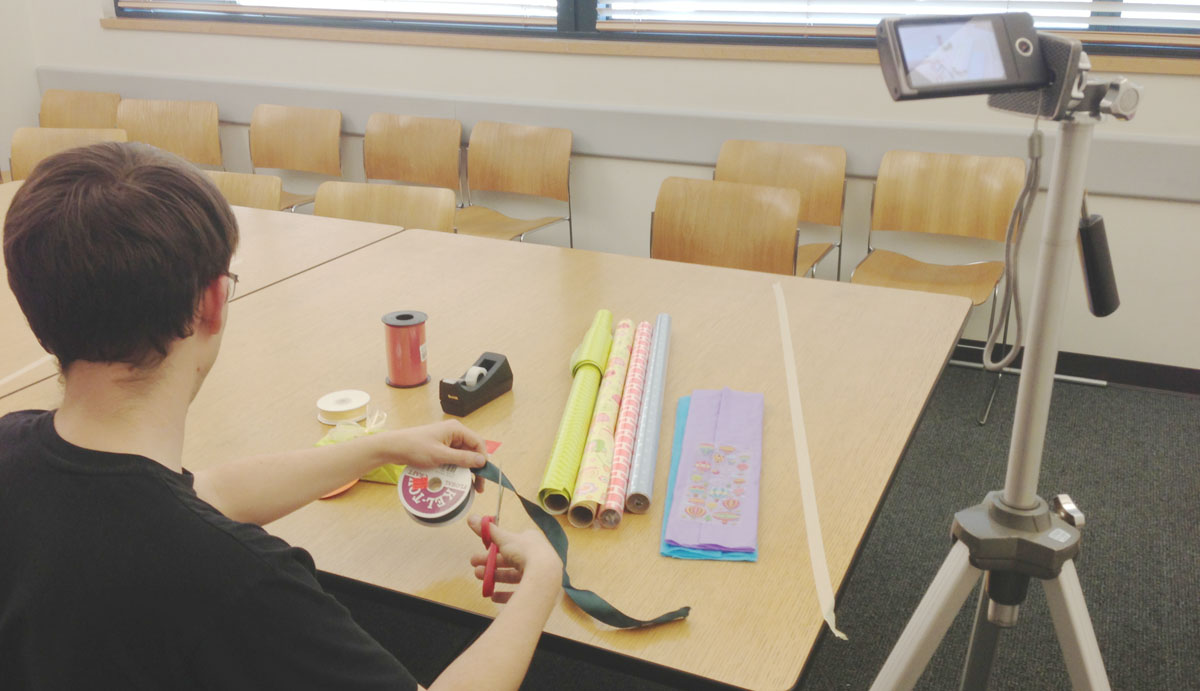
\includegraphics[width=0.6\columnwidth]{\democut/fig/eval-setup}
  \caption{Our user study setup}
  \label{fig:eval-setup}
\end{figure}


%\subsection{Participants}
%We recruited 8 participants (4 males aged 22-41 and 4 females aged 20-33) who were either university students or employees of a local software company.
%We sent invitations to a campus student design group and a software design company to visit our lab and create a video instructional tutorial \iquote{How to Wrap a Gift.}
%We recruited 8 participants (Z males, aged P-Q),
%, and compensated each with a \$25 gift card for participating.
%We balanced recruitment such that
%Half of our participants had prior video editing experience, while the other half were video editing novices.
%Half of the participants had created tutorials before, in any format and topic. To help them understand the context, candidates were asked to watch three online video before visiting our lab. The three videos were selected from the formative user study and included topics of repair, cooking, and electronics.

\subsubsection{Procedure and Environment}
The study was conducted in a quiet lab environment with static lighting. We used a tripod-mounted Sony camcorder to record the gift wrapping task (Figure~\ref{fig:eval-setup}), and a Macbook Pro running OS X and Google Chrome for DemoCut. The laptop was connected to a 30-inch monitor and external mouse and keyboard. Each study session lasted 60-90 minutes.

\subsubTitleBold{Introduction (15 minutes)} The participants viewed a web-based tutorial that introduced the goal and procedure of the study. In the tutorial, the participants practiced annotating a one-minute demo video with five types of markers, reviewed a system-generated result, and modified video effects in the DemoCut Editing interface.

\subsubTitleBold{Filming setup and practice (5 minutes)} The participants were asked to plan their gift-wrapping demonstration with any of the provided supplies. The camcorder was positioned either opposite the participants or behind them on the right and was angled down to capture their workspace on a conference table. The participants reviewed the camera's point of view and were told that any activities outside of the delineated workspace would not be captured. The participants were free to plan their task on paper or conduct a practice run. %They were allowed to change the viewpoint upon requests, write down a plan on paper, and practice if needed.

\subsubTitleBold{Filming demonstration (10-20 minutes)} The participants filmed their gift wrapping demonstration in a single take. The study moderator initiated and terminated the recording, but did not provide additional assistance.

\subsubTitleBold{Annotating and editing (30-45 minutes)} The participants annotated their video with the DemoCut Annotation Interface and modified the generated video tutorial using the DemoCut Editing Interface.

\subsubTitleBold{Review of the final video and discussion (10 minutes)} Finally, participants reviewed the final video, completed a questionnaire, and discussed the process with experimenters.
